\documentclass[11pt]{scrartcl}
\usepackage{dominatrix}
\usepackage{solarized-light}
\lstset{
language=R
}
\renewcommand\thesection{Problem \arabic{section}}
\renewcommand\thesubsection{\thesection (\alph{subsection})}
\renewcommand\thesubsubsection{(\roman{subsubsection})}

\newcommand{\portfolio}[2]{\ensuremath{\dfrac{K_3-K_2}{K_3-K_1}#1 + \dfrac{K_2-K_1}{K_3-K_1}#2}}
\newcommand{\leftportfolio}[1]{\ensuremath{\dfrac{K_3-K_2}{K_3-K_1}#1}}

\newcommand{\defrac}[2]{\ensuremath{\frac{\delta #1}{\delta #2}}}
\newcommand{\dedefrac}[2]{\ensuremath{\frac{\delta^2 #1}{\delta #2^2}}}
\newcommand{\dededefrac}[3]{\ensuremath{\frac{\delta^2 #1}{\delta #2 \delta #3}}}
\renewcommand{\sf}{\ensuremath{Se^{(r-q)(T-t)}}}

\newcommand{\epower}[1]{\ensuremath{e^{\left(#1\right)}}}


\title{Homework 8}
\subject{Intro to Financial Engineering IEOR W4700}
\author{Linan Qiu\\\texttt{lq2137}}
\begin{document}
\maketitle

\section{}

\[\Gamma = \dedefrac{C}{S} = \frac{\epower{-\frac{d_1^2}{2}}}{S\sigma\sqrt{2\pi t}}\]

Now,

\[\defrac{d_1}{S} = \frac{1}{S\sigma\sqrt{t}}\]

Then, at maximum $\Gamma$,

\begin{align*}
\defrac{\Gamma}{S} &= \frac{-\epower{-\frac{d_1^2}{2}}}{S^2\sigma\sqrt{2\pi t}} - \frac{\epower{-\frac{d_1^2}{2}}}{S\sigma\sqrt{2\pi t}} d_1 \defrac{d_1}{S} \\
&= \frac{-\epower{-\frac{d_1^2}{2}}}{S^2\sigma\sqrt{2\pi t}} \left(1 + \frac{d_1}{\sigma \sqrt{t}} \right) = 0 \\
-1 &= \frac{d_1}{\sigma\sqrt{t}} = \frac{\log{\left(\frac{S}{Ke^{-rt}}\right)} + 0.5\sigma^2 t}{\sigma^2 t}
\end{align*}

Solving for $S$,

\begin{align*}
-\sigma^2 t - 0.5 \sigma^2 t &= \log{\left( \frac{S}{Ke^{-rt}} \right)} \\
&= \log{S} - \log{K} + rt \\
-1.5\sigma^2 t - rt + \log{K} &= \log{S} \\
S &= K\epower{-(1.5\sigma^2+r)t}
\end{align*}

\section{}

The value of a put option can be calculated via:

\begin{lstlisting}
d1 = function(S, K, r, sigma, T) {
  return((log(S/K) + (r+(sigma^2)/2)*T)/(sigma*sqrt(T)))
}

d2 = function(S, K, r, sigma, T) {
  return(d1(S, K, r, sigma, T) - sigma*sqrt(T))
}

bsm_put = function(sigma, K, S, r, T) {
  d1_val = d1(S, K, r, sigma, T)
  d2_val = d2(S, K, r, sigma, T)
  return(price=K*exp(-r*T)*pnorm(-d2_val) - S*pnorm(-d1_val))
}
\end{lstlisting}

Given a quoted price, we want to find the value of \texttt{sigma} that makes \texttt{bsm\_put} equal to the quoted price.

\begin{lstlisting}
sigma_root_put = function(sigma, S, K, r, T, price) {
  return(bsm_put(sigma=sigma, K=K, S=S, r=r, T=T) - price)
}
\end{lstlisting}

This can be done via \texttt{uniroot} in \texttt{R}

\begin{lstlisting}
implied_volatility_put = function(S, K, r, T, price) {
  return(uniroot(sigma_root_put, c(-10^99, 10^99), S=S, K=K, r=r, T=T, price=price)$root)
}
\end{lstlisting}

Solving the problem and plotting is then trivial:

\begin{lstlisting}
strike = c(91:110)
putprice = c(9.57,9.78,10.01,10.24,10.49,10.75,
   11.02,11.31,11.61,11.92,12.25,12.60,12.96,
   13.344,13.74,14.16,14.60,15.05,15.53,16.02)
volatility = mapply(implied_volatility_put, K=strike, price=putprice, S=100, r=0, T=1)

library(ggplot2)

data = as.data.frame(list(strike=strike, volatility=volatility))
plot = ggplot(data=data) + geom_line(aes(x=strike, y=volatility)) + geom_point(aes(x=strike, y=volatility)) + labs(title="Implied Volatility Smile", x="Strike Price", y="Implied Volatility")
\end{lstlisting}

\begin{figure}[H]
\centering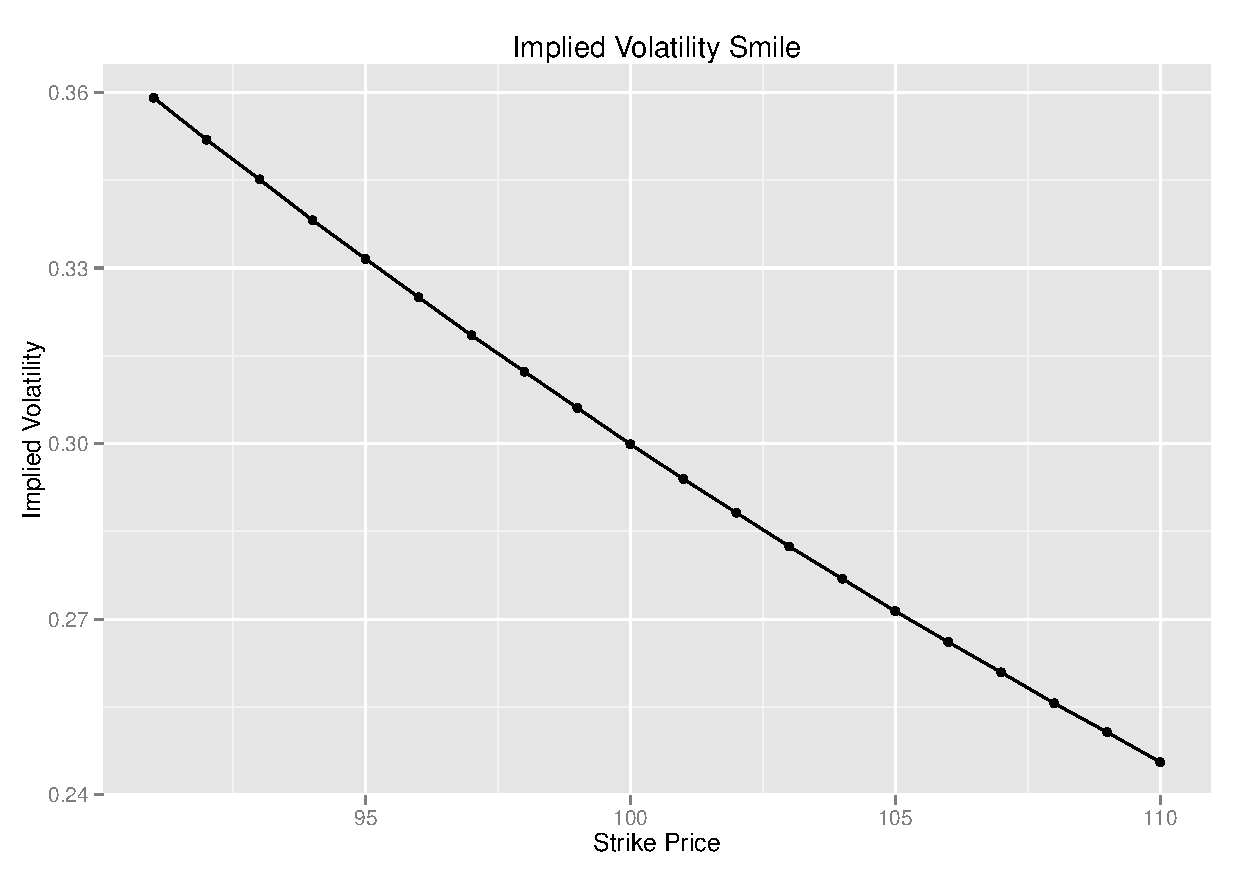
\includegraphics[width=\textwidth]{./hw8/implied_volatility.pdf}
\caption{Plot of implied volatility against strike price.}
\end{figure}

\section{}

Let $\pi$ be the value of the portfolio. Then $\Delta \Pi$ is the price change of the portfolio. Assume that the volatility of the underlying asset $S$ is constant. Then, Taylor series expansion gives

\[\Delta \Pi = \defrac{\Pi}{S} \Delta S + \defrac{\Pi}{t} \Delta t + \frac{1}{2}\dedefrac{\Pi}{S} \Delta S^2 + \frac{1}{2}\dedefrac{\Pi}{t}\Delta t^2 + \dededefrac{\Pi}{S}{t} \Delta S \Delta t + ...\]

If the portfolio $\Pi$ is delta-hedged, the first term $\defrac{\Pi}{S}\Delta S$ is eliminated. The second term, $\Theta = \defrac{\Pi}{t}$ is non stochastic. Hence for a delta neutral portfolio,

\[\Delta \Pi = \Theta \Delta t + \frac{1}{2}\Gamma \Delta S^2\]

when terms of order higher than $\Delta t$ are ignored.

For a portfolio that is only long call / put, the delta of the portfolio is always increasing as $S$ increases, hence $\Gamma \geq 0$. Then, when $\Delta S$ is greater, $\Delta \Pi$ is greater and hence profits are greater. Hence, wild movements in exchange rates will be more profitable than virtually constant exchange rates if the portfolio is perfectly delta hedged.

\section{}

Data entry intern task.

\begin{lstlisting}
positions = c(-5000, -500, -2000, -500)
deltas = c(0.5, 0.7, -0.4, 0.7)
gammas = c(2.2, 0.6, 1.3, 1.9)
vegas = c(1.8, 0.2, 0.8, 1.4)
to_delta = 0.7
to_gamma = 1.4
to_vega = 0.9
sterling_delta = 1
sterling_gamma = 0
sterling_vega = 0
\end{lstlisting}

\subsection{}

Let $w_t$ be position in traded option and $w_s$ be position in sterling.

To make the portfolio delta neutral,

\[w_t 0.7 + w_s = -\sum_{i \in \mathrm{OTCs}} w_i * \Delta_i\]

To make the portfolio gamma neutral we note that the $\Gamma$ of sterling is 0, since sterling's $\Delta$ is always 1,

\[w_t 1.4 = -\sum_{i \in \mathrm{OTCs}} w_i * \Gamma_i\]

To solve this,

\begin{lstlisting}
> # delta gamma
> # solve a %*% x = b
> b = c(-sum(positions*deltas), -sum(positions*gammas))
> a = matrix(c(to_delta, to_gamma, sterling_delta, sterling_gamma), nrow=2, ncol=2)
> colnames(a) = c('traded_option', 'sterling')
> rownames(a) = c('delta', 'gamma')
> a
      traded_option sterling
delta           0.7        1
gamma           1.4        0
> solve(a, b)
traded_option      sterling 
     10607.14      -5025.00 
\end{lstlisting}

\subsection{}

To make portfolio delta neutral,

\[w_t 0.7 + w_s = -\sum_{i \in \mathrm{OTCs}} w_i * \Delta_i\]


To make portfolio vega\footnote{I forgot for a moment that finance is weird and Vega is totally not a Greek letter. \LaTeX{} gave me an error when I tried to type \texttt{\textbackslash Vega}} neutral we note that sterling's $\kappa$ is always 0 since the value of the asset does not change with volatility,

\[w_t 0.9 = -\sum_{i \in \mathrm{OTCs}} w_i * \kappa_i\]

To solve this,

\begin{lstlisting}
> # delta vega
> # solve a %*% x = b
> b = c(-sum(positions*deltas), -sum(positions*gammas))
> a = matrix(c(to_delta, to_vega, sterling_delta, sterling_vega), nrow=2, ncol=2)
> colnames(a) = c('traded_option', 'sterling')
> rownames(a) = c('delta', 'vega')
> a
      traded_option sterling
delta           0.7        1
vega            0.9        0
> solve(a, b)
traded_option      sterling 
        16500         -9150 
\end{lstlisting}

\section{}

\begin{table}[H] \centering
\begin{tabu}{cccccc}
\toprule
t & Stock Price & Delta & Shares Purchased & Cost of Shares & Cash Position \\
\midrule
Setup & - & - & - & - & -20.510 \\
\midrule
0.000 & 100.000 & 0.750 & -0.750 & -75.000 & 54.490 \\
0.250 & 116.180 & 0.890 & -0.140 & -16.265 & 72.415 \\
0.500 & 100.000 & 0.710 & 0.180 & 18.000 & 56.620 \\
0.750 & 86.070 & 0.190 & 0.520 & 44.756 & 13.588 \\
1.000 & 100.000 & 1.000 & -0.810 & -81.00 & \textbf{95.002} \\
\bottomrule
\end{tabu}
\end{table}

In the final period, we exercise the option at receive \$5. This leaves us with \$100.002 in cash. Then, we close out the long position of $\Delta_{1} = 1$ shares (technically we could have just not longed 0.81 shares in the last period and closed out the short position, but I did this to stick with the example in the slides and also for clarity, assuming 0 transaction costs). The closing out reduces cash by $\$-100.000$, resulting in remaining cash of $\$0.002$, reasonably close to zero.

Since we could not make money by delta hedging, the \$20.51 price for the option was fair given the parameters and trees provided.



\end{document}